% Options for packages loaded elsewhere
\PassOptionsToPackage{unicode}{hyperref}
\PassOptionsToPackage{hyphens}{url}
%
\documentclass[
]{article}
\usepackage{amsmath,amssymb}
\usepackage{iftex}
\ifPDFTeX
  \usepackage[T1]{fontenc}
  \usepackage[utf8]{inputenc}
  \usepackage{textcomp} % provide euro and other symbols
\else % if luatex or xetex
  \usepackage{unicode-math} % this also loads fontspec
  \defaultfontfeatures{Scale=MatchLowercase}
  \defaultfontfeatures[\rmfamily]{Ligatures=TeX,Scale=1}
\fi
\usepackage{lmodern}
\ifPDFTeX\else
  % xetex/luatex font selection
\fi
% Use upquote if available, for straight quotes in verbatim environments
\IfFileExists{upquote.sty}{\usepackage{upquote}}{}
\IfFileExists{microtype.sty}{% use microtype if available
  \usepackage[]{microtype}
  \UseMicrotypeSet[protrusion]{basicmath} % disable protrusion for tt fonts
}{}
\makeatletter
\@ifundefined{KOMAClassName}{% if non-KOMA class
  \IfFileExists{parskip.sty}{%
    \usepackage{parskip}
  }{% else
    \setlength{\parindent}{0pt}
    \setlength{\parskip}{6pt plus 2pt minus 1pt}}
}{% if KOMA class
  \KOMAoptions{parskip=half}}
\makeatother
\usepackage{xcolor}
\usepackage[margin=1in]{geometry}
\usepackage{graphicx}
\makeatletter
\def\maxwidth{\ifdim\Gin@nat@width>\linewidth\linewidth\else\Gin@nat@width\fi}
\def\maxheight{\ifdim\Gin@nat@height>\textheight\textheight\else\Gin@nat@height\fi}
\makeatother
% Scale images if necessary, so that they will not overflow the page
% margins by default, and it is still possible to overwrite the defaults
% using explicit options in \includegraphics[width, height, ...]{}
\setkeys{Gin}{width=\maxwidth,height=\maxheight,keepaspectratio}
% Set default figure placement to htbp
\makeatletter
\def\fps@figure{htbp}
\makeatother
\setlength{\emergencystretch}{3em} % prevent overfull lines
\providecommand{\tightlist}{%
  \setlength{\itemsep}{0pt}\setlength{\parskip}{0pt}}
\setcounter{secnumdepth}{-\maxdimen} % remove section numbering
% definitions for citeproc citations
\NewDocumentCommand\citeproctext{}{}
\NewDocumentCommand\citeproc{mm}{%
  \begingroup\def\citeproctext{#2}\cite{#1}\endgroup}
\makeatletter
 % allow citations to break across lines
 \let\@cite@ofmt\@firstofone
 % avoid brackets around text for \cite:
 \def\@biblabel#1{}
 \def\@cite#1#2{{#1\if@tempswa , #2\fi}}
\makeatother
\newlength{\cslhangindent}
\setlength{\cslhangindent}{1.5em}
\newlength{\csllabelwidth}
\setlength{\csllabelwidth}{3em}
\newenvironment{CSLReferences}[2] % #1 hanging-indent, #2 entry-spacing
 {\begin{list}{}{%
  \setlength{\itemindent}{0pt}
  \setlength{\leftmargin}{0pt}
  \setlength{\parsep}{0pt}
  % turn on hanging indent if param 1 is 1
  \ifodd #1
   \setlength{\leftmargin}{\cslhangindent}
   \setlength{\itemindent}{-1\cslhangindent}
  \fi
  % set entry spacing
  \setlength{\itemsep}{#2\baselineskip}}}
 {\end{list}}
\usepackage{calc}
\newcommand{\CSLBlock}[1]{\hfill\break\parbox[t]{\linewidth}{\strut\ignorespaces#1\strut}}
\newcommand{\CSLLeftMargin}[1]{\parbox[t]{\csllabelwidth}{\strut#1\strut}}
\newcommand{\CSLRightInline}[1]{\parbox[t]{\linewidth - \csllabelwidth}{\strut#1\strut}}
\newcommand{\CSLIndent}[1]{\hspace{\cslhangindent}#1}
\usepackage{booktabs}
\usepackage{longtable}
\usepackage{array}
\usepackage{multirow}
\usepackage{wrapfig}
\usepackage{float}
\usepackage{colortbl}
\usepackage{pdflscape}
\usepackage{threeparttable}
\usepackage{threeparttablex}
\usepackage[normalem]{ulem}
\usepackage{makecell}
\usepackage{xcolor}
\ifLuaTeX
  \usepackage{selnolig}  % disable illegal ligatures
\fi
\usepackage{bookmark}
\IfFileExists{xurl.sty}{\usepackage{xurl}}{} % add URL line breaks if available
\urlstyle{same}
\hypersetup{
  pdftitle={HCD Simulations Write Up},
  pdfauthor={Audrey Fu Lab},
  hidelinks,
  pdfcreator={LaTeX via pandoc}}

\title{HCD Simulations Write Up}
\author{Audrey Fu Lab}
\date{14 January, 2025}

\begin{document}
\maketitle

\section*{Data Simulation}\label{data-simulation}
\addcontentsline{toc}{section}{Data Simulation}

\subsubsection*{Simulating networks}\label{simulating-networks}
\addcontentsline{toc}{subsubsection}{Simulating networks}

We adopt a top-down approach to simulate hierarchical networks,
considering various simulation parameters such as graph sparsity, noise,
and the architecture of the super-level graph(s), including small-world,
scale-free, and random graph networks (Watts and Strogatz 1998; Barabási
and Bonabeau 2003).

Our simulations focus on basic hierarchies comprising one or two
hierarchical layers. Two-layer networks mirror classical community
detection on graphs, where our aim is to recover the true community
labels from a given graph. Meanwhile, three-layer networks present a
more intricate scenario, where the bottom layer of the hierarchy
contains two levels of community structure. Here, the top level
corresponds to the nodes at the uppermost layer of the hierarchy, and
the middle level consists of communities nested within the top-level
communities. The objective with these networks is to identify both sets
of community partitions.

In each hierarchy, for fully connected networks, we initiate by
simulating \(N_{\text{top}}\) top-level nodes, adhering to a directed
small-world, random graph, or scale-free network architecture (Watts and
Strogatz 1998; Barabási and Bonabeau 2003). In cases where the network
is disconnected, we simply simulate \(N_{\text{top}}\) disconnected
nodes. For networks with three hierarchical layers, we then generate a
subnetwork of \(N_{\text{middle}}\) nodes from each top-layer node,
adhering to the network structure utilized at the top level. If the
network is fully connected, we apply a probability \(p_\text{between}\)
to the nodes from different top-level communities being connected.

The final step in all hierarchies is to generate the nodes in the
observed (bottom) layer of the hierarchy. For each top-layer or
middle-layer node, we generate a sub-network of \(N_{\text{bottom}}\)
nodes under the same sub-network structure as the previous layers, and
we apply a probability \(p_\text{between}\) for nodes from different
communities to share an edge.

\subsubsection*{Simulating gene
expression}\label{simulating-gene-expression}
\addcontentsline{toc}{subsubsection}{Simulating gene expression}

Once we simulate a hierarchical graph, we utilize this hierarchy to
generate the node-feature matrix, which depicts the expression of \(N\)
genes across \(d\) samples. Here, \(N\) denotes the number of nodes in
the observed (bottom) layer of the hierarchy.

We simulate the node-feature matrix using the topological order of the
observed level graph. We start by generating the features of nodes that
have no parental input. We refer to these nodes as \emph{origin} nodes.
All origin nodes are simulated from a normal distribution with mean
\(0\) and standard deviation \(\sigma\). All other nodes are simulated
from a normal distribution centered at the mean of their parent nodes
and with standard deviation \(\sigma\).

\section*{Hierarchical Commuity Detection (HCD)
Overview}\label{hierarchical-commuity-detection-hcd-overview}
\addcontentsline{toc}{section}{Hierarchical Commuity Detection (HCD)
Overview}

Our HCD method consists of two modules:

\begin{enumerate}
\def\labelenumi{\arabic{enumi}.}
\item
  A graph autoencoder based on the architecture proposed by Salehi and
  Davulcu (2019) which utilizes graph attention layers such as those
  first introduced by Veličković et al. (2017) (See most recent version
  of pseudocode for details). In our applications, we incorporate
  multi-head attention in all encoder and decoder layers to expand model
  learning capacity. The graph autoencoder module takes a set of node
  attributes \({\bf X}\in\mathbb{R}^{N \times d}\) and an adjacency
  matrix \({\bf A}_{ij}\in[0,1]\) defining the relationships between the
  node as input and learns a low dimensional embedding
  \({\bf Z} \in \mathbb{R}^{N \times q}\) of the network and attributes.
  This embedding is then used to reconstruct the node attributes and
  adjacency matrix under a separate loss function for each.
\item
  The second module of HCD takes the embeddings \({\bf Z}\) generated by
  the autoencoder and applies a multilevel community detection process.
  This module first applies the function \(f_{top}\) which partitions
  the data into \(k\) groups. The function \(f_{top}\) can be either (i)
  the \(SoftKMeans\) layer described by {[}@{]} or a neural layer such
  as
\end{enumerate}

\[f_{top}({\bf Z}) = \theta({\bf ZW} + {\bf b})\] The above example is a
simple fully connected layer where
\({\bf W} \in \mathbb{R}^{N \times k}\) is a matrix of parameters,
\({\bf b} \in \mathbb{R}^N\) is a bias parameter vector and \(\theta\)
is an activation function such as the \(ReLU\) function. Alternative
types of layer can also be used such the GraphSAGE convolution described
by {[}@{]} or graph attention.

\section{Simulations}\label{simulations}

Here we describe the settings for three different sets of simulations.
For each set of simulations, we simulated hierarchical gene networks
consisting of 5 top level nodes/communities, 15 middle level
nodes/communities and 300 nodes/genes at the observed level of the
hierarchy. We simulate networks for all three graph types (small world,
scale free or random graph) with the nodes at the top level of the
hierarchy either all connected or all disconnected. We also simulated
nodes under two levels of noise with noise set to either
\(\sigma = 0.1\) or \(\sigma = 0.5\). Additionally, we sample the
probability for edges within and between node communities at the middle
layer and bottom level from the uniform distributions

\begin{tabular}{lllrr}
\toprule
Layer & Connection & Sampling Distibution & Lower Bound & Upper Bound\\
\midrule
Middle & Within & Uniform & 0.010 & 0.15\\
 & Between & Uniform & 0.010 & 0.15\\
Bottom & Within & Uniform & 0.001 & 0.05\\
 & Between & Uniform & 0.001 & 0.05\\
\bottomrule
\end{tabular}

Each combination of parameters (graph type, connectivity, and noise) is
replicated multiple times.

\section{Set 1 Simulations}\label{set-1-simulations}

In this set of simulations, the HCD model uses a linear neural layer for
both the top and middle layer partitions. For these experiments, we set
the output size of each neural network to match the ground truth (i.e.,
output size of 5 for the top layer and 15 for the middle layer). Unlike
classical hierarchical clustering, where setting \(k\) identifies the
``best'' cut of the dendrogram to find \(k\) communities, setting the
output size to the ground truth for the neural network predictors does
not guarantee they will predict exactly 5 or 15 communities. Instead, it
sets an upper bound on the number of communities that may be found. A
comprehensive list of parameter settings is outlined in the table below.

\begin{table}
\centering
\caption{\label{tab:paramtab1}Simulation Set 1 model parameter settings}
\centering
\begin{tabular}[t]{l|l}
\hline
Parameter & Value\\
\hline
patience & 10\\
\hline
method & top down\\
\hline
batch learning & TRUE\\
\hline
batch\_size & 64\\
\hline
AE operator & GATv2Conv\\
\hline
COMM operator & Linear\\
\hline
attn. heads & 5\\
\hline
dropout & 0.2\\
\hline
Layer Normalization & TRUE\\
\hline
AE hidden sizes & [256, 128]\\
\hline
Comm output size (Top) & 5\\
\hline
Comm output size (Middle) & 15\\
\hline
\$\textbackslash{}gamma\$ & 1\\
\hline
\$\textbackslash{}delta\$ & 1\\
\hline
\$\textbackslash{}lambda\$ & [1, 1]\\
\hline
learning rate & 0.001\\
\hline
Max epochs & 200\\
\hline
Graph correlation cutoff & 0.2\\
\hline
\% Training & 80\\
\hline
\% Testing & 20\\
\hline
\end{tabular}
\end{table}

\section{Set 2 Simulations}\label{set-2-simulations}

In Set 2 of our simulations, we apply HCD using the same model and
network simulation settings as Set 1, which are outlined in
\textbf{Tables} @ref(tab:paramtab1) - @ref(tab:simtab1). However, in
this scenario, we investigate HCD's performance on complex networks with
approximately 1,000 nodes in the hierarchy's bottom layer.

\begin{longtable}[t]{ll}
\caption{\label{tab:unnamed-chunk-1}Model Parameter Settings}\\
\toprule
Parameter & Value\\
\midrule
patience & 10\\
method & top down\\
batch learning & TRUE\\
batch\_size & 64\\
AE operator & GATv2Conv\\
\addlinespace
COMM operator & Linear\\
attn. heads & 5\\
dropout & 0.2\\
Layer Normalization & TRUE\\
AE hidden sizes & {}[256, 128]\\
\addlinespace
Comm output size (Top) & 5\\
Comm output size (Middle) & 15\\
\$\textbackslash{}gamma\$ & 1\\
\$\textbackslash{}delta\$ & 1\\
\$\textbackslash{}lambda\$ & {}[1, 1]\\
\addlinespace
learning rate & 0.001\\
Max epochs & 200\\
Graph correlation cutoff & 0.2\\
\% Training & 80\\
\% Testing & 20\\
\bottomrule
\end{longtable}

\section{Set 3 Simulations}\label{set-3-simulations}

\subsubsection*{Evaluating performance}\label{evaluating-performance}
\addcontentsline{toc}{subsubsection}{Evaluating performance}

We evaluate the performance of our HCD method using three graph-based
clustering metrics:

\begin{enumerate}
\def\labelenumi{\arabic{enumi}.}
\item
  \textbf{homogeneity} evaluates the degree to which each predicted
  community contains only data points from a single true community,
  indicating how well the algorithm avoids mixing different groups.
  Thus, homogeneity tends to be high if resolved communities contain
  only members of the same true community.
\item
  \textbf{completeness} assesses the extent to which all data points
  that belong to the same true community are correctly assigned to a
  single predicted community. Thus completeness is always high if all
  members of the same true communities end up in the same resolved
  community even if several true communities are allocated together.
\item
  \textbf{NMI} Normalized Mutual Information (NMI) is a weighted average
  of the Completeness and Homogeneity two metrics.
\item
  \textbf{ARI} The Adjusted Rand Index (ARI) is a metric that measures
  the similarity between two different clusterings of the same data,
  correcting for the chance of random agreement. It ranges from -1 to 1,
  where 1 indicates perfect agreement between the clusterings, 0
  represents random labeling, and negative values indicate less
  agreement than expected by chance.
\end{enumerate}

In all simulations we compare HCD with two commonly used heuristic
methods:

\begin{itemize}
\item
  \textbf{Louvain Method}: This widely used community detection
  algorithm optimizes modularity by iteratively reassigning nodes
  between communities and merging communities. It automatically
  determines the number of communities and is highly efficient for
  processing large networks. In all simulations, we apply the Louvain
  method to the estimated adjacency matrix, which is derived from the
  correlation matrix of the node features. The resulting community
  predictions are compared to the ground truth for both the top and
  middle layers of the simulated hierarchy.
\item
  \textbf{Hierarchical Clustering using Ward's Distance (HC)}: This
  agglomerative clustering approach iteratively merges clusters to
  minimize the increase in within-cluster variance. Ward's method tends
  to produce compact, spherical clusters and generates a dendrogram
  representing the full hierarchical structure of the data. In all
  simulations, HC is applied to the simulated gene expression data (node
  feature matrix). The optimal community predictions are determined by
  identifying the best cutting point on the dendrogram, aligning with
  the ground truth clusters (five clusters and 15 clusters).
\end{itemize}

\subsubsection{Points to investigate}\label{points-to-investigate}

\begin{figure}
\centering
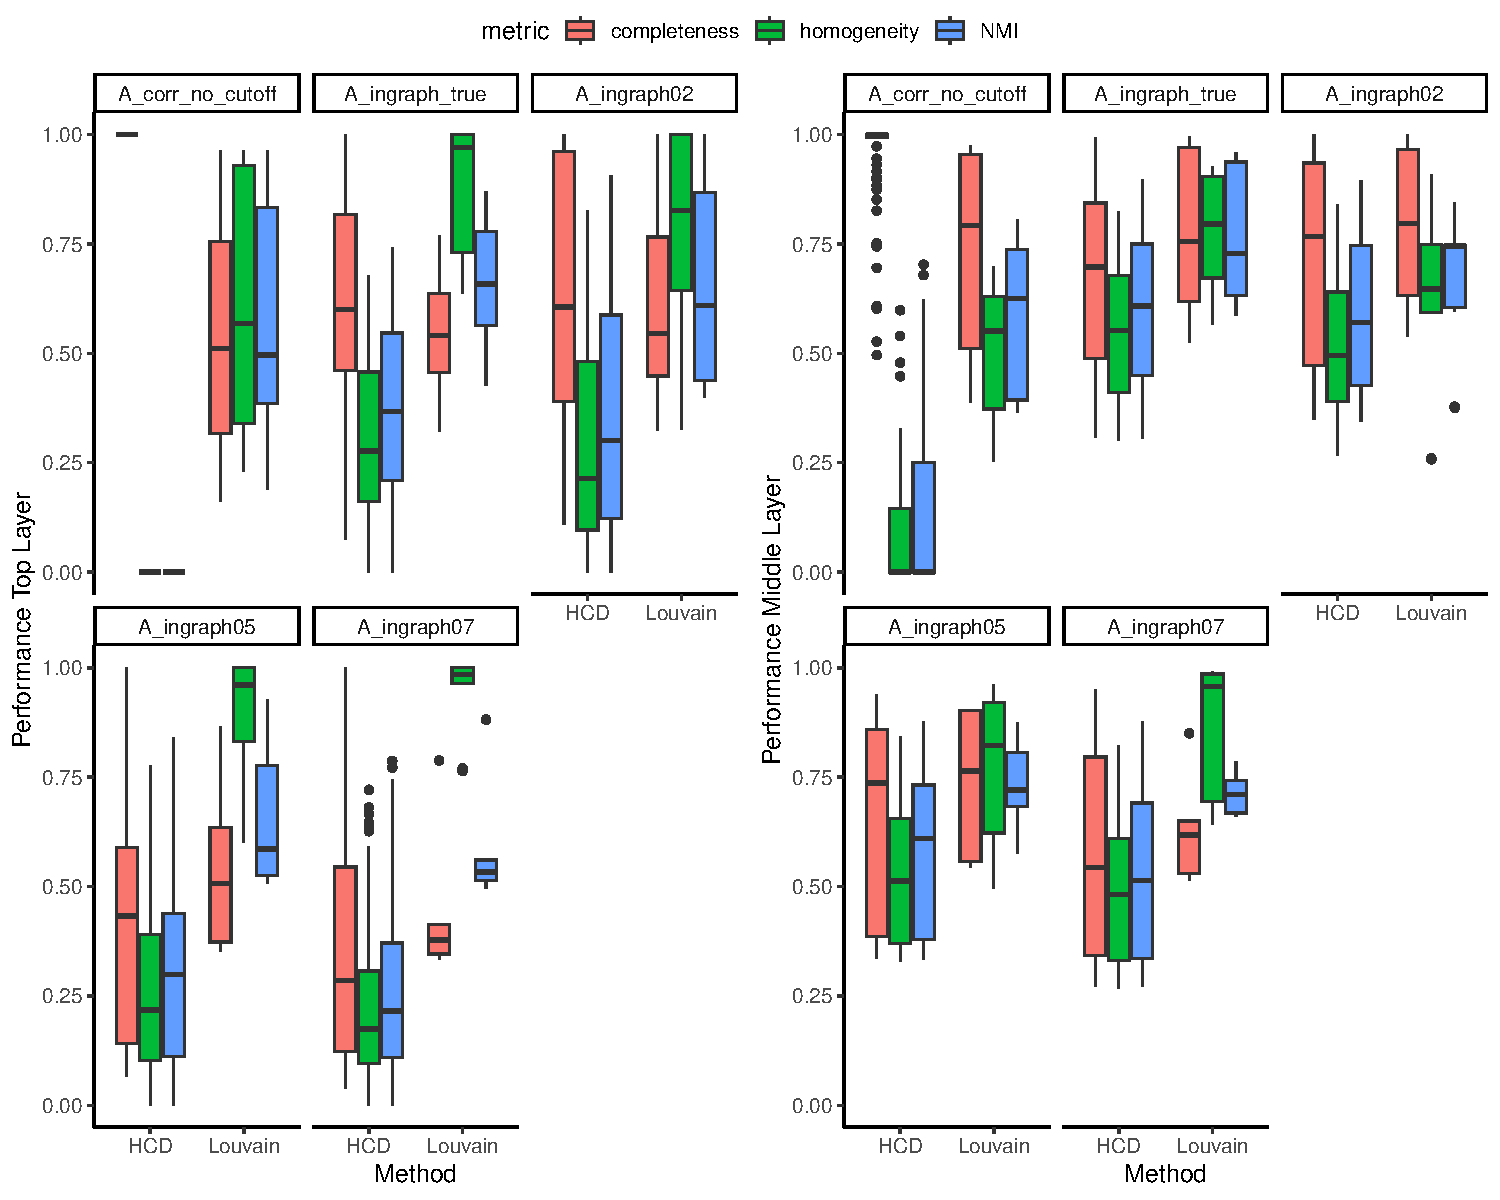
\includegraphics{report_12_18_2024_files/figure-latex/unnamed-chunk-3-1.pdf}
\caption{Hierarchical clustering performance for the top layer of the
hierarchical for HCD, classical hierarchical clustering using Ward's
Distance (HC) and the Louvain method. Each point represents the
performance in homogeneity and completeness for a unique simulated
hierarchy. The diagonal line represents 1 to 1 corresponds between
completeness and homogeneity. Points that fall above the line represent
clustering solutions that overgroup the true communities while points
that fall below the line represent clusters that break up the true
communities. Points on the diagonal line represent a better clustering
solution}
\end{figure}

\begin{figure}
\centering
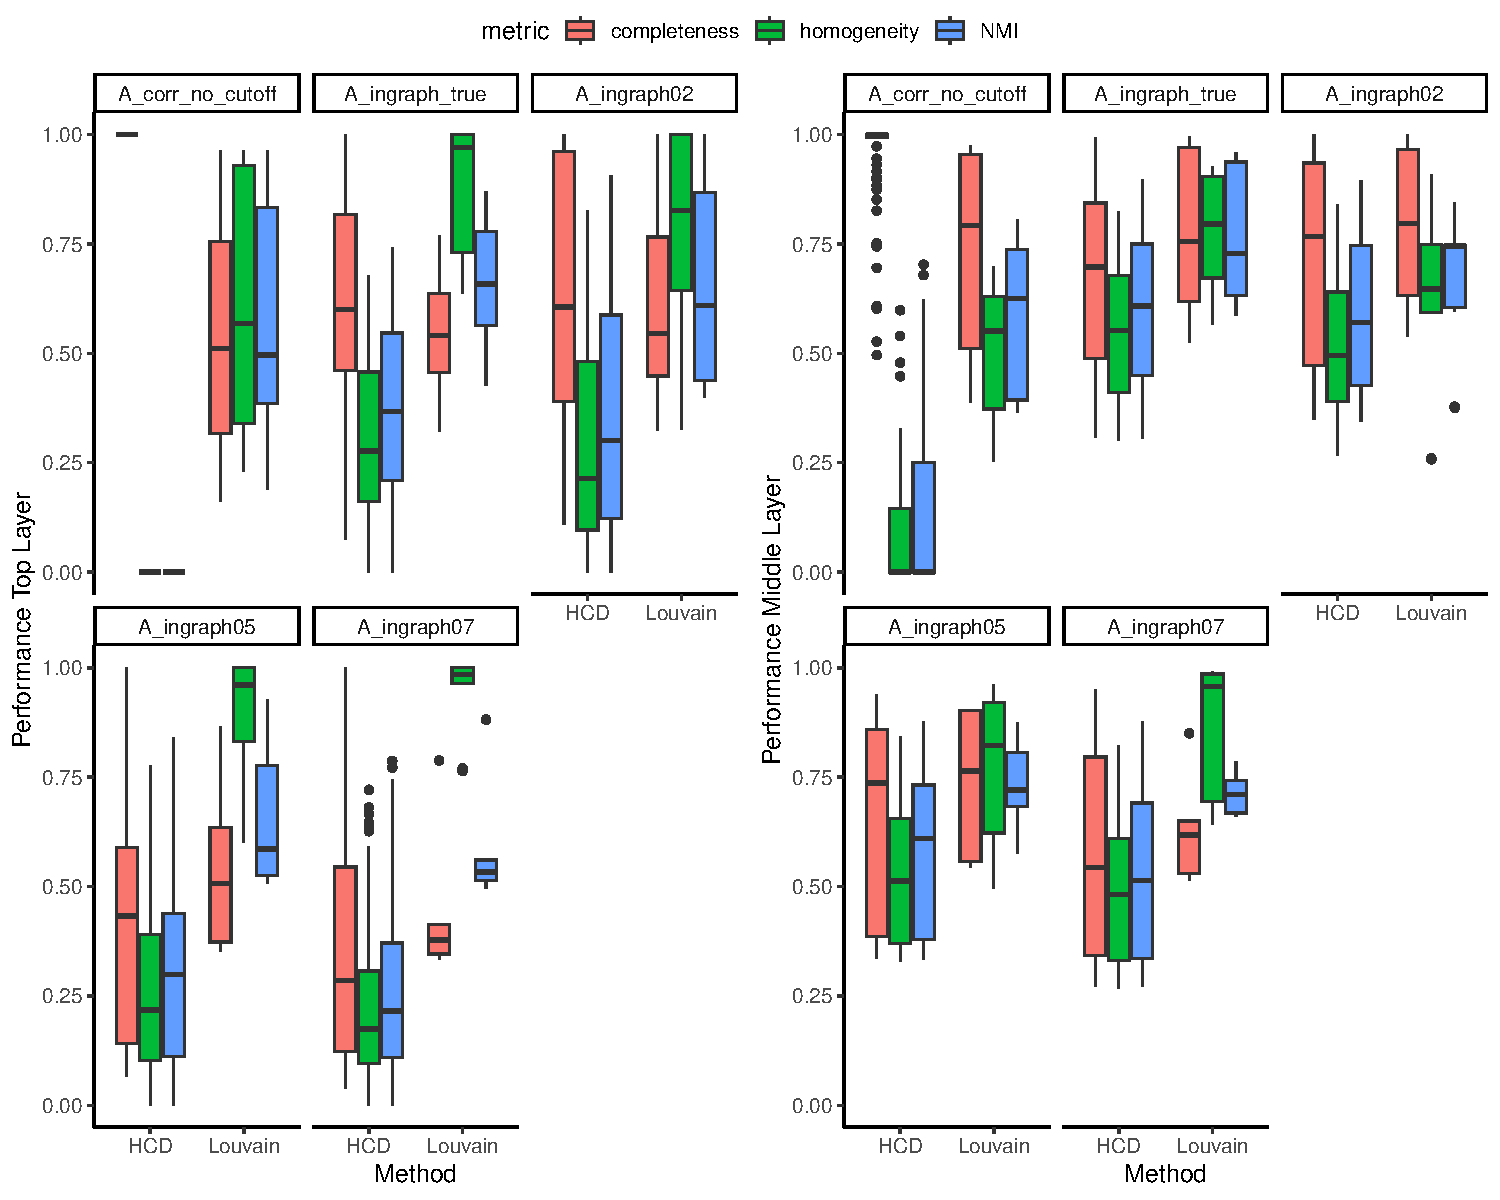
\includegraphics{report_12_18_2024_files/figure-latex/unnamed-chunk-4-1.pdf}
\caption{Hierarchical clustering performance for the middle layer of the
hierarchical for HCD, classical hierarchical clustering using Ward's
Distance (HC) and the Louvain method. Each point represents the
performance in homogeneity and completeness for a unique simulated
hierarchy. The diagonal line represents 1 to 1 corresponds between
completeness and homogeneity. Points that fall above the line represent
clustering solutions that overgroup the true communities while points
that fall below the line represent clusters that break up the true
communities. Points on the diagonal line represent a better clustering
solution.}
\end{figure}

\section{complex networks}\label{complex-networks}

\begin{figure}
\centering
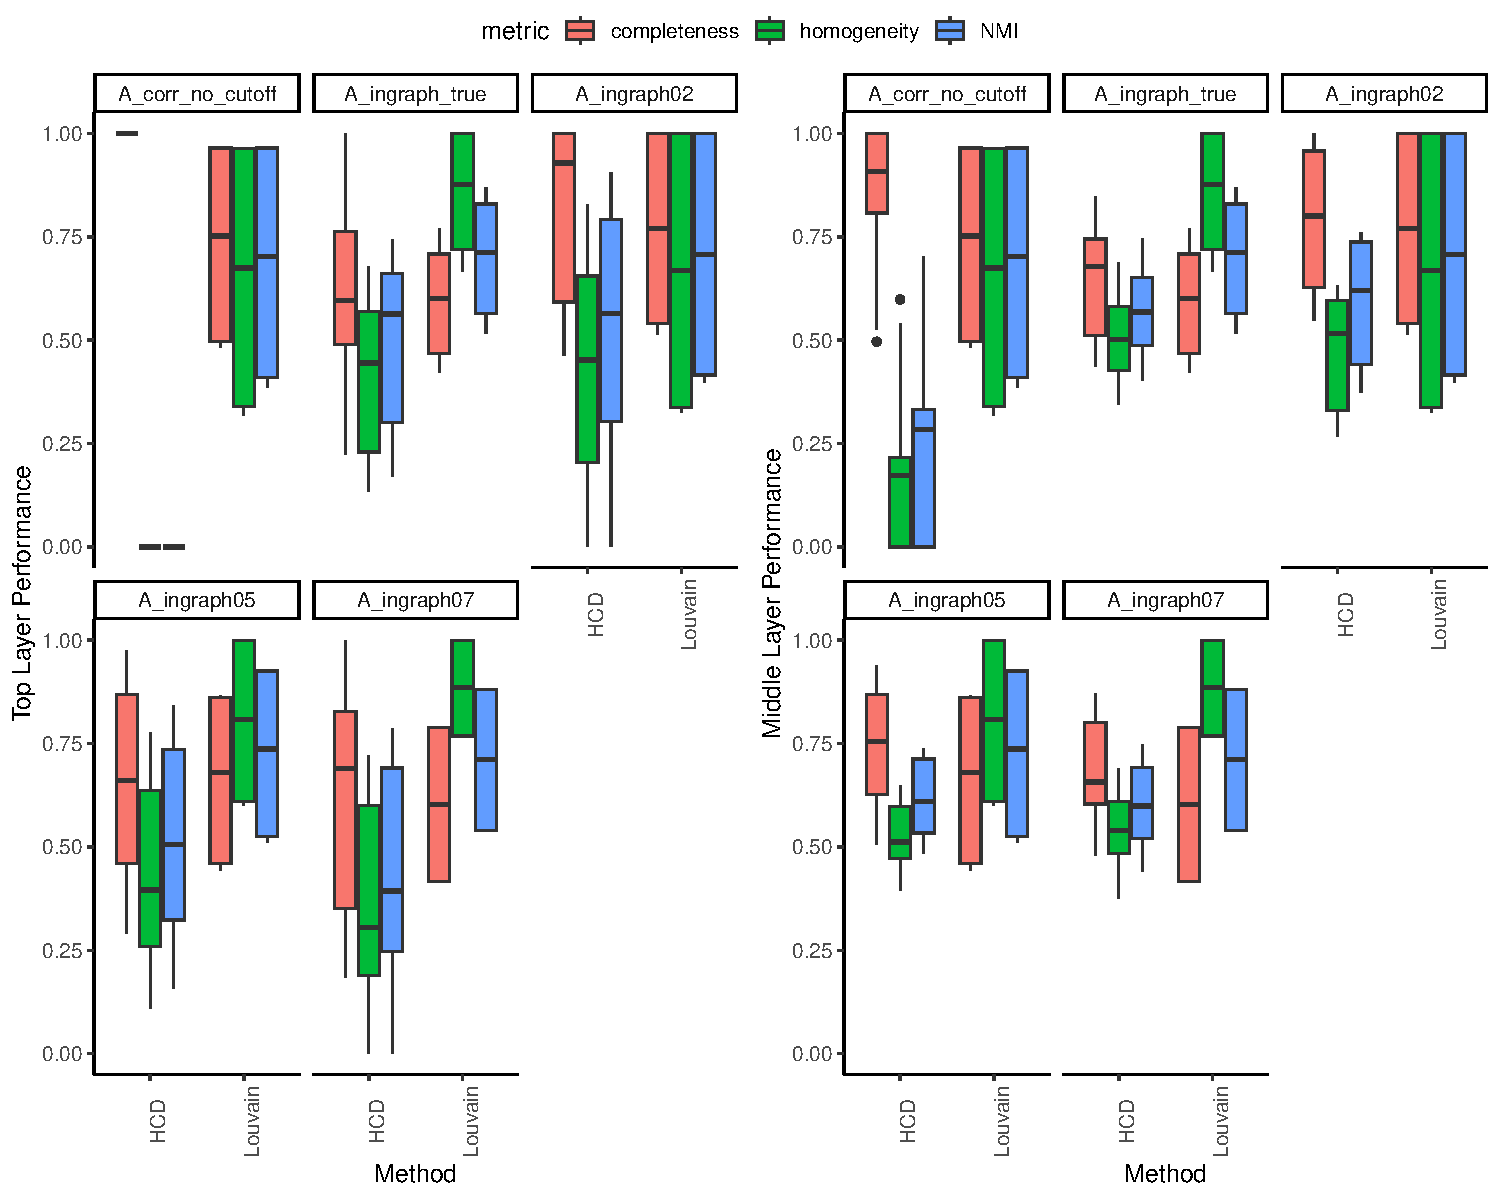
\includegraphics{report_12_18_2024_files/figure-latex/unnamed-chunk-6-1.pdf}
\caption{Hierarchical clustering performance for the top layer of the
hierarchical for HCD, classical hierarchical clustering using Ward's
Distance (HC) and the Louvain method. Each point represents the
performance in homogeneity and completeness for a unique simulated
hierarchy. The diagonal line represents 1 to 1 corresponds between
completeness and homogeneity. Points that fall above the line represent
clustering solutions that overgroup the true communities while points
that fall below the line represent clusters that break up the true
communities. Points on the diagonal line represent a better clustering
solution}
\end{figure}

\begin{figure}
\centering
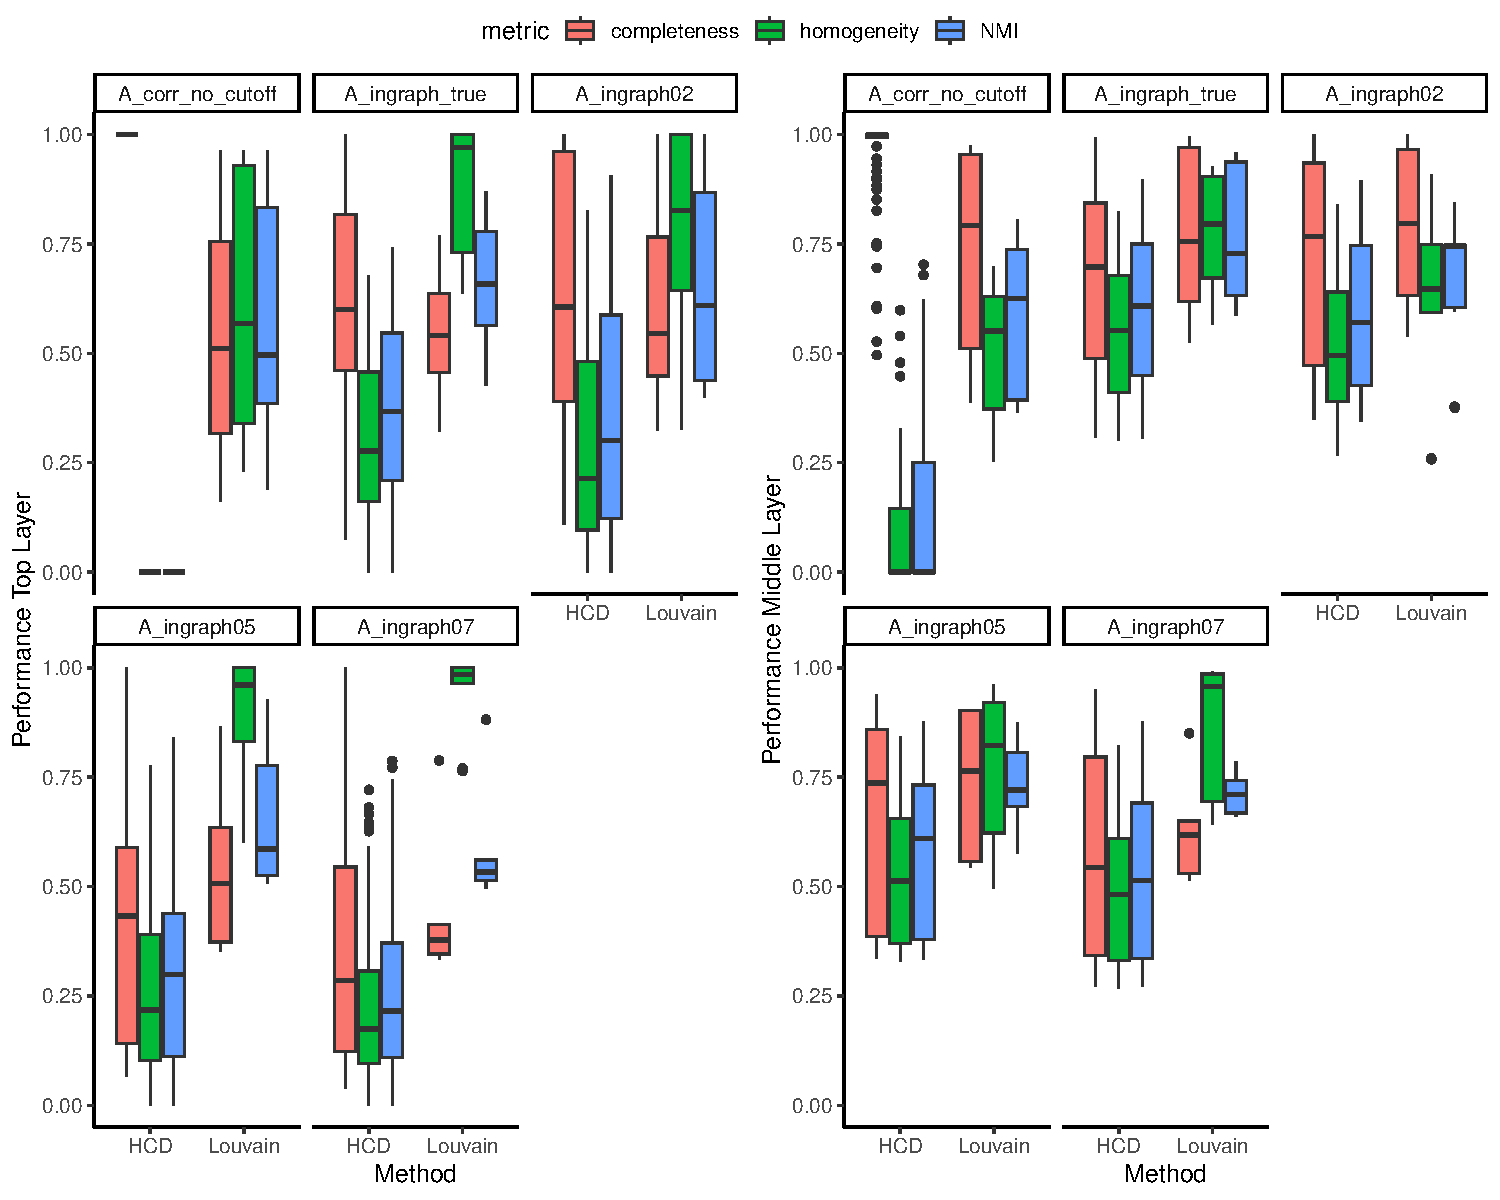
\includegraphics{report_12_18_2024_files/figure-latex/unnamed-chunk-7-1.pdf}
\caption{Hierarchical clustering performance for the middle layer of the
hierarchical for HCD, classical hierarchical clustering using Ward's
Distance (HC) and the Louvain method. Each point represents the
performance in homogeneity and completeness for a unique simulated
hierarchy. The diagonal line represents 1 to 1 corresponds between
completeness and homogeneity. Points that fall above the line represent
clustering solutions that overgroup the true communities while points
that fall below the line represent clusters that break up the true
communities. Points on the diagonal line represent a better clustering
solution.}
\end{figure}

\phantomsection\label{refs}
\begin{CSLReferences}{1}{0}
\bibitem[\citeproctext]{ref-barabasi2003scale}
Barabási, Albert-László, and Eric Bonabeau. 2003. {``Scale-Free
Networks.''} \emph{Scientific American} 288 (5): 60--69.

\bibitem[\citeproctext]{ref-salehi2019graph}
Salehi, Amin, and Hasan Davulcu. 2019. {``Graph Attention
Auto-Encoders.''} \emph{arXiv Preprint arXiv:1905.10715}.

\bibitem[\citeproctext]{ref-velivckovic2017graph}
Veličković, Petar, Guillem Cucurull, Arantxa Casanova, Adriana Romero,
Pietro Lio, and Yoshua Bengio. 2017. {``Graph Attention Networks.''}
\emph{arXiv Preprint arXiv:1710.10903}.

\bibitem[\citeproctext]{ref-watts1998collective}
Watts, Duncan J, and Steven H Strogatz. 1998. {``Collective Dynamics of
`Small-World'networks.''} \emph{Nature} 393 (6684): 440--42.

\end{CSLReferences}

\end{document}
